\documentclass[a4paper]{article}
\usepackage{WUSTReport}
\usepackage{hyperref}
\usepackage{nameref}
\usepackage{natbib}
\usepackage{siunitx}
\usepackage{todonotes}

\sisetup{
  per-mode=symbol
}

\title{Optical Fibers and Optocommunication --- Laboratory 3: Optical Time-Domain Reflectometry (OTDR)}
\author{Kamil Czop 259613\\Sergiusz Warga 230757}
\date{}
\reportgroup{Even Monday 13:15}
\reporttutor{dr inż.~Paweł Kaczmarek}

\makeatletter
% define a macro \Autoref to allow multiple references to be passed to \autoref
\newcommand\Autoref[1]{\@first@ref#1,@}
\def\@throw@dot#1.#2@{#1}% discard everything after the dot
\def\@set@refname#1{%    % set \@refname to autoefname+s using \getrefbykeydefault
    \edef\@tmp{\getrefbykeydefault{#1}{anchor}{}}%
    \xdef\@tmp{\expandafter\@throw@dot\@tmp.@}%
    \ltx@IfUndefined{\@tmp autorefnameplural}%
         {\def\@refname{\@nameuse{\@tmp autorefname}s}}%
         {\def\@refname{\@nameuse{\@tmp autorefnameplural}}}%
}
\def\@first@ref#1,#2{%
  \ifx#2@\autoref{#1}\let\@nextref\@gobble% only one ref, revert to normal \autoref
  \else%
    \@set@refname{#1}%  set \@refname to autoref name
    \@refname~\ref{#1}% add autoefname and first reference
    \let\@nextref\@next@ref% push processing to \@next@ref
  \fi%
  \@nextref#2%
}
\def\@next@ref#1,#2{%
   \ifx#2@ and~\ref{#1}\let\@nextref\@gobble% at end: print and+\ref and stop
   \else, \ref{#1}% print  ,+\ref and continue
   \fi%
   \@nextref#2%
}
\makeatother

\begin{document}
\maketitle

\section{Optical Time-Domain Reflectometry}
Note that the magnitude of the step is twice that of the splice loss, since light scattered from locations behind the splice will experience that last twice --- on the forward and backward pass.~\cite{RP:OTDR}

\section{Laboratory routine and equipment}
The laboratory routine was to investigate different optical fiber spools with the Grandway FHO5000 Optical Time-Domain Reflectometer.
Between the spools and the reflectometer, there was a 1 km start-up optical fiber that was supposed to serve as a reference.

Throughout the laboratory, we measured the following optical fiber spools:
\begin{enumerate}
    \item 3M Optical Fiber Power-Core, seen in~\autoref{fig:spool-1}.
    \item SM-EYOF-7/130 SM Erbium-Ytterbium Double Clad Fiber
    \item FiberHome Non-Zero Dispersion-Shifted Single-Mode Optical Fiber (G.655)
    \item Some mysterious spool.
\end{enumerate}
All of the spools were terminated with FC/APC connectors.
We investigated the connectors for dust before connecting.
If necessary, we cleaned them with the fiber cleaning cloth spool.

\begin{figure}
    \centering
    \includegraphics[width=0.7\textwidth]{images/OTDR-Setup.pdf}
    \caption{The optical link setup for Optical Time-Domain Reflectometry.
        All the parts are connected via FC connectors}%
    \label{fig:OTDR-Setup}
\end{figure}

\begin{figure}
    \centering
    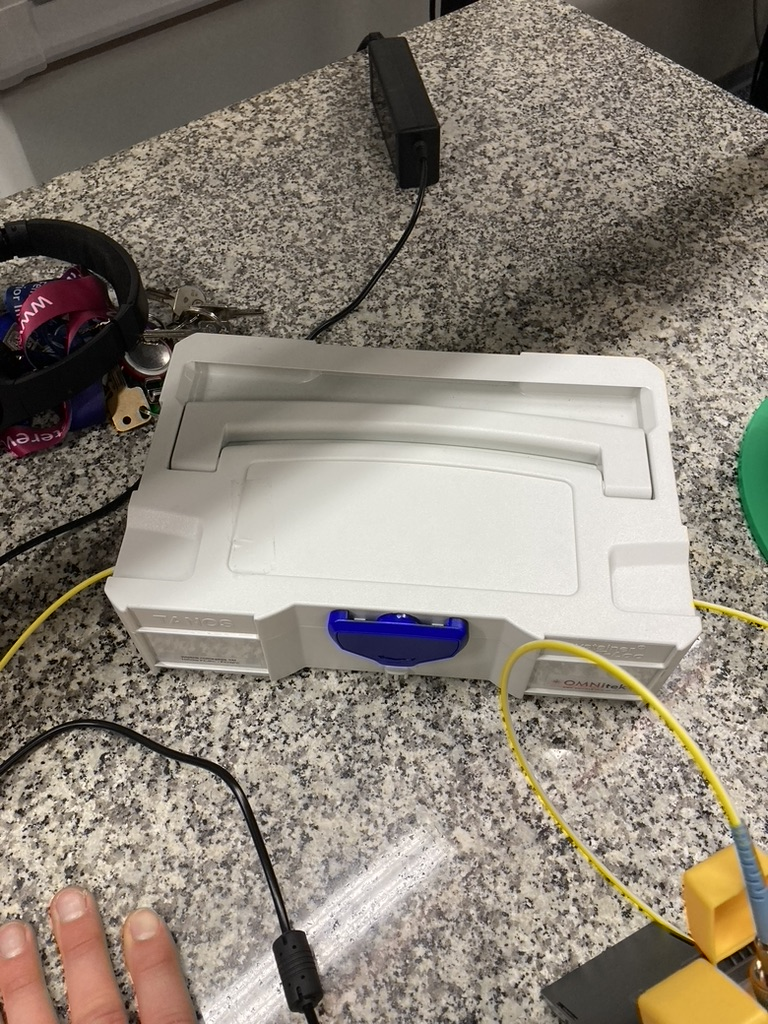
\includegraphics[width=0.7\textwidth]{images/start-up_fibre.jpeg}
    \caption{1km start-up optical fiber in a case}%
    \label{fig:start-up_fibre}
\end{figure}

\begin{figure}
    \centering
    \includegraphics[width=0.7\textwidth]{images/OTDR-Spool_1.png}
    \caption{The first optical fiber spool's label. The ''200'' on the label \textit{may} indicate its core diameter to be \qty{200}{\um}}%
    \label{fig:spool-1}
\end{figure}

\section{Measurements}
The OTDRViewer automatically found and clustered the events.
\subsection{Start-Up fibre}
At the beginning we connected the 1 km start-up fiber and ran the analysis to obtain a reference measurement, seen in~\autoref{fig:start-up_fibre}.
Unfortunatelly, we performed the analysis for the $\lambda=\qty{1310}{\nm}$ only.

\begin{figure}
    \centering
    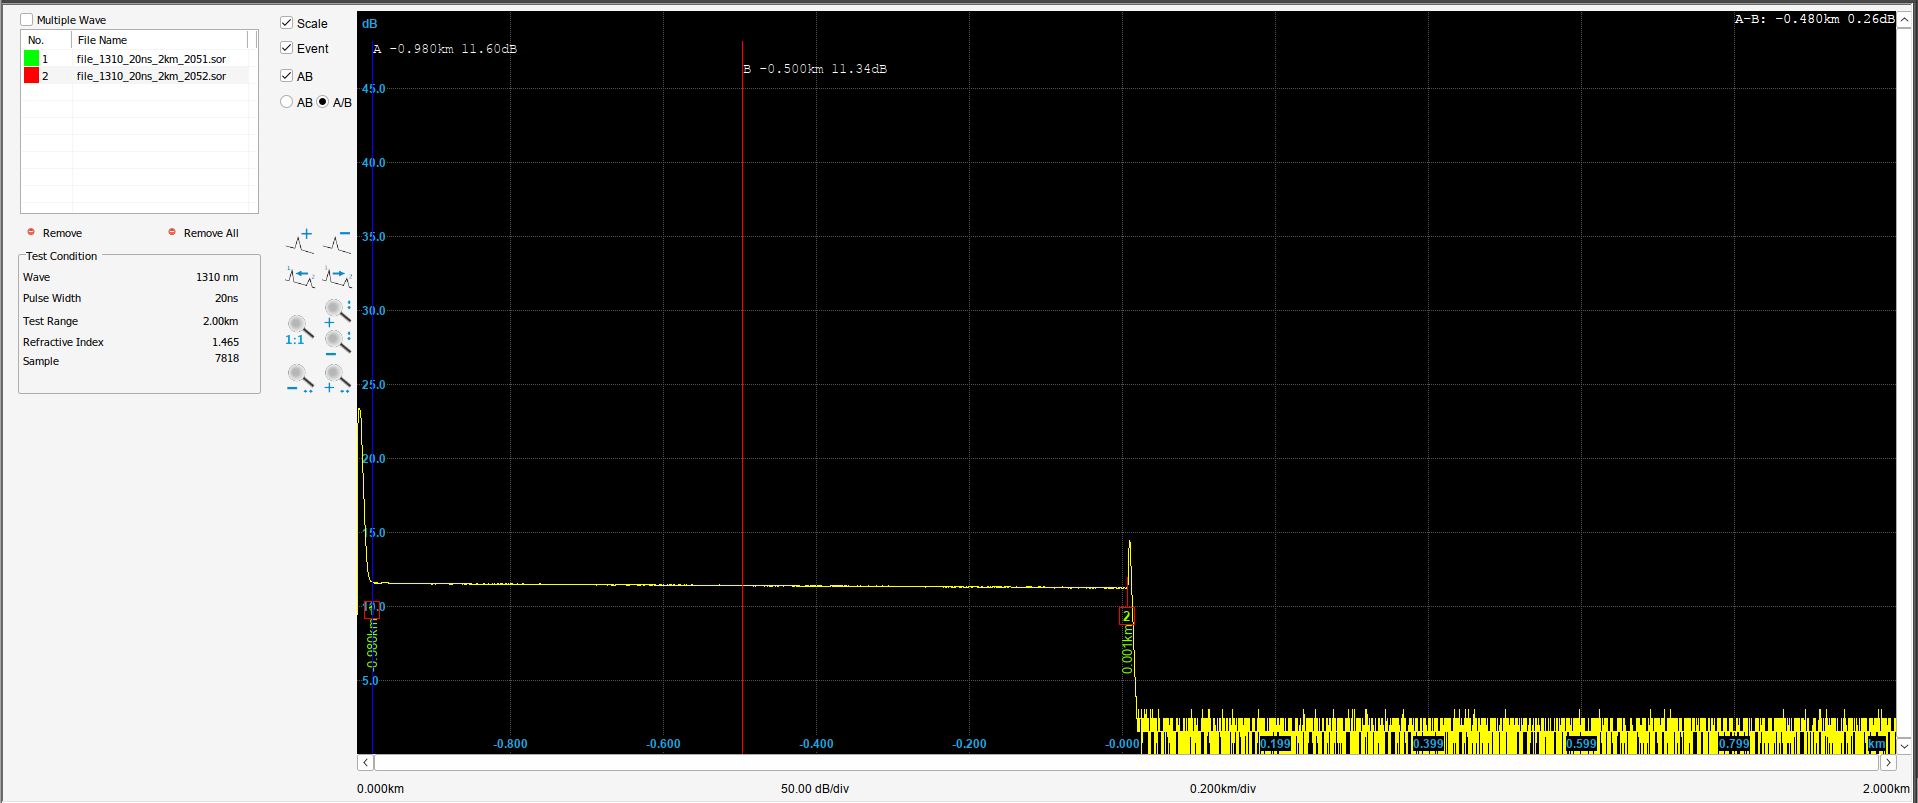
\includegraphics[width=0.7\textwidth]{images/OTDRViewer_Start-Up}
    \label{fig:OTDRViewer_start-up_fibre}
\end{figure}

\subsection{3M Optical Fiber Power-Core}

The first spool seen in~\autoref{fig:spool-1} was labeled with the length of \qty{3}{\km}.
The OTDRViewer analysis restults may be seen in~\Autoref{fig:OTDRViewer-spool_1-1310nm-20ns.png,fig:OTDRViewer-spool_1-1550nm-20ns.png}.
Two observed events are the connection between the start-up fiber and the spool, and the loose connector reflection.
The measured fibre attenuation was \qty{0.649}{\dB\per\km} for \qty{1310}{\nm} and \qty{0.358}{\dB\per\km} for \qty{1550}{\nm}.

\begin{figure}
    \centering
    \includegraphics[width=\textwidth]{images/OTDRViewer-spool_1-1310nm-20ns.png}
    \caption{OTDRViewer analysis of the first spool ran at \qty{1310}{\nm} with \qty{20}{\ns} pulse}%
    \label{fig:OTDRViewer-spool_1-1310nm-20ns.png}
\end{figure}

\begin{figure}
    \centering
    \includegraphics[width=\textwidth]{images/OTDRViewer-spool_1-1550nm-20ns.png}
    \caption{OTDRViewer analysis of the first spool ran at \qty{1550}{\nm} with \qty{20}{\ns} pulse}%
    \label{fig:OTDRViewer-spool_1-1550nm-20ns.png}
\end{figure}

Oh boi.

\todo[inline]{Embed measurements}
\todo[inline]{Determine the length of a fiber and its attenuation or unit attenuation (dB/km) for every span of fiber measured.}
\todo[inline]{Present the reflectometer trace for long distance, multisegment link, showing appropriate spools measured before, compare segments parameters with those measured before}
\todo[inline]{Mark and calculate the parameters of each fiber connection in that “link” (localization, attenuation)}
\todo[inline]{Compare the results for both wavelengths used}
\todo[inline]{Explain all the artefacts and unexpected events on your link trace.}

\bibliographystyle{alpha}
\bibliography{bibliography}

\end{document}
